\section{Eigenfaces}
\label{sec:intro}

Face data is the base dataset for our experiment. This consists of 520 data with 52 classes and 10 data for each class. We will conduct the upcoming experiments by dividing the data for each class into an 8:2 train-test split.

%-------------------------------------------------------------------------
\subsection{Eigenfaces}

There are two method to conduct PCA: PCA($S=AA^T$) and low dimensional PCA($S=A^TA$). We compare two methods on training dataset with size 2576*416(D*N).

\begin{figure}[htbp]
	\centering
	\begin{subfigure}[t]{0.48\linewidth}
		\centering
		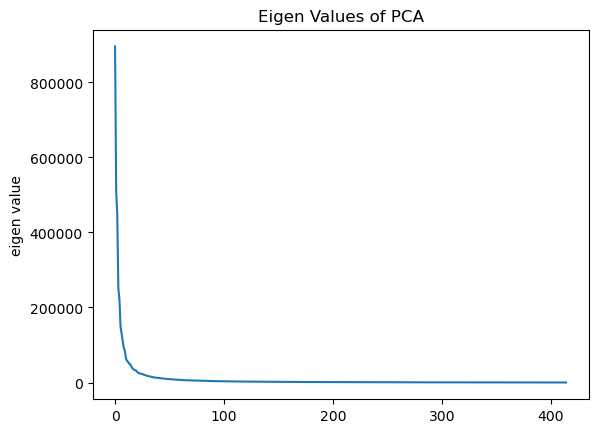
\includegraphics[width=\linewidth]{image/q1_eigval_pca.png}
		\caption{nonzero eigenvalues of PCA}
		\label{fig:eigval_pca}
	\end{subfigure}%
	\hfill
	\begin{subfigure}[t]{0.48\linewidth}
		\centering
		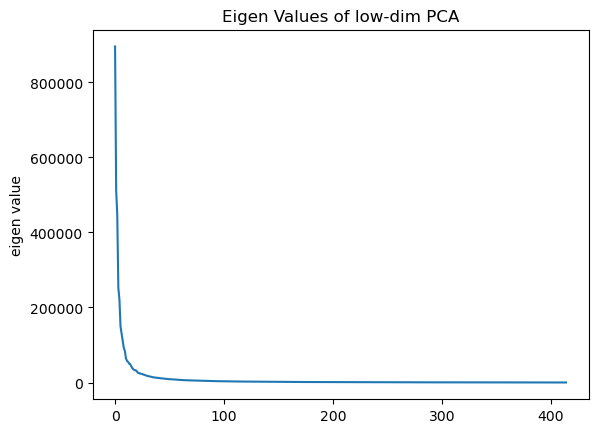
\includegraphics[width=\linewidth]{image/q1_eigval_lowdim.png}
		\caption{nonzero eigenvalues of low-dimensional PCA}
		\label{fig:eigval_lowdim}
	\end{subfigure}
	\caption{Comparison between eigenvalues of PCA methods}
	\label{fig:q1_eigval}
\end{figure}

As shown in \cref{fig:q1_eigval} both methods have the same nonzero eigenvalues. Specifically, PCA has 2576 nonzero eigenvalues, and low-dimensional PCA has 416. However, when selecting values bigger than $\frac{1}{100}$, both methods yield 415 eigenvalues. This is because, given matrix sizes of 2576x2576 and 416x416, the maximum ranks are 2576 and 416, respectively. But since we have 416 data points, the PCA projection subspace can at most capture 415 meaningful dimensions, resulting in 415 eigenvalues larger than $\frac{1}{100}$. From this comparison (\cref{fig:q1_eigval}), we conclude that both methods yield the same eigenvalues, and their top 415 eigenvectors are also identical.

The only difference between them is computation time: PCA takes 8.015s, while low-dimensional PCA takes 1.092s. Low-dimensional PCA is faster because, in our case, the data dimension exceeds the number of data points, making its covariance matrix smaller than that of PCA. Based on this time efficiency, we use low-dimensional PCA going forward. % 시간복잡도는 O(N^3)인데 이것보단 적게 차이나는데 어쩌지!!


\subsection{Image reconstuction using Eigenfaces}
Using pca basis from above, we perform face reconstruction. \cref{fig:recon_train} and \cref{fig:recon_test} shows reconstruction results using different numbers of PCA bases. As seen in the images, the reconstruction become more accurate with more bases. When using only 10 bases, the results resemble the mean face(\cref{fig:q1_meanface}) of training data. This occurs because the PCA basis is oriented to capture common features by maximizing data variance. Thus, with a small number of bases, the reconstruction reflects common features of the dataset more strongly than specific details of each image.

\begin{figure}
	\centering
	\begin{subfigure}[t]{0.2\linewidth}
		\centering
		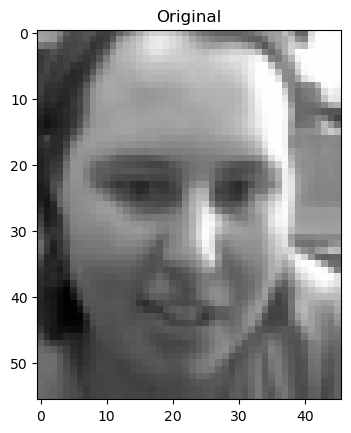
\includegraphics[width=\linewidth]{image/q1_recon_train_original.png}
		\caption{original}
		\label{fig:train_re_original}
	\end{subfigure}%
	\hfill
	\begin{subfigure}[t]{0.2\linewidth}
		\centering
		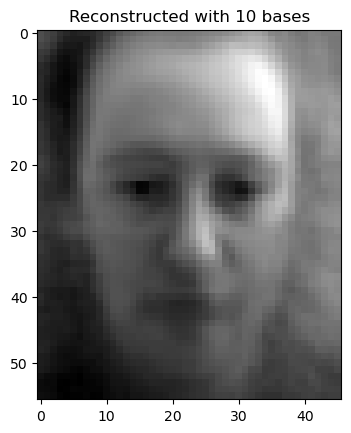
\includegraphics[width=\linewidth]{image/q1_recon_train_10.png}
		\caption{10 bases}
		\label{fig:train_re_10}
	\end{subfigure}
    \hfill
	\begin{subfigure}[t]{0.2\linewidth}
		\centering
		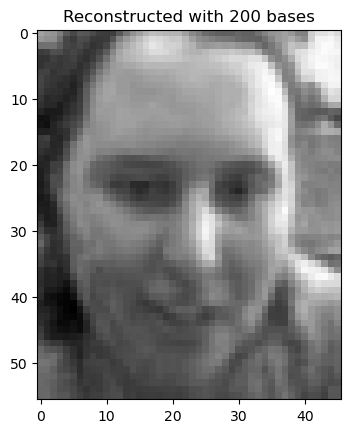
\includegraphics[width=\linewidth]{image/q1_recon_train_200.png}
		\caption{200 bases}
		\label{fig:train_re_200}
	\end{subfigure}
    \hfill
	\begin{subfigure}[t]{0.2\linewidth}
		\centering
		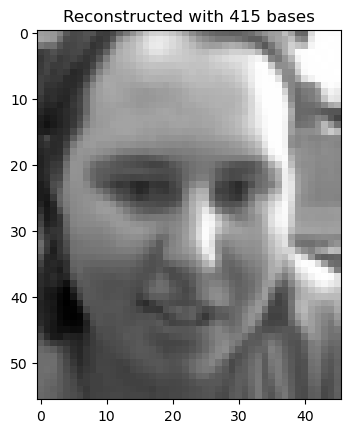
\includegraphics[width=\linewidth]{image/q1_recon_train_415.png}
		\caption{415 bases}
		\label{fig:train_re_415}
	\end{subfigure}
	\caption{Training data reconstruction results}
	\label{fig:recon_train}
\end{figure}

\begin{figure}
	\centering
	\begin{subfigure}[t]{0.2\linewidth}
		\centering
		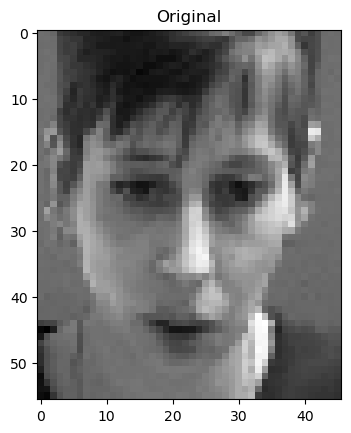
\includegraphics[width=\linewidth]{image/q1_recon_test_original.png}
		\caption{original}
		\label{fig:test_re_original}
	\end{subfigure}%
	\hfill
	\begin{subfigure}[t]{0.2\linewidth}
		\centering
		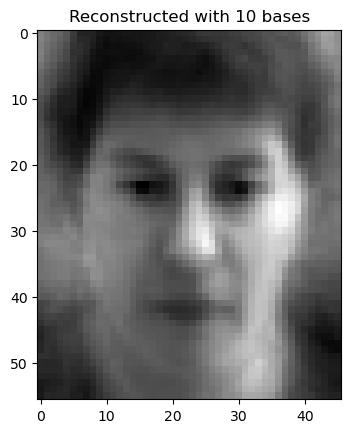
\includegraphics[width=\linewidth]{image/q1_recon_test_10.png}
		\caption{10 bases}
		\label{fig:test_re_10}
	\end{subfigure}
    \hfill
	\begin{subfigure}[t]{0.2\linewidth}
		\centering
		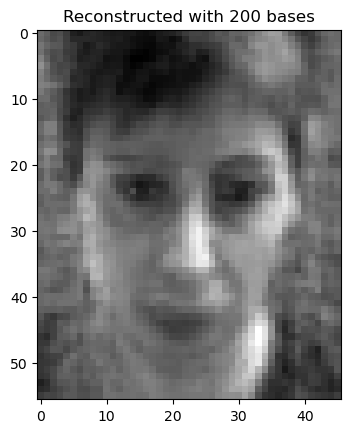
\includegraphics[width=\linewidth]{image/q1_recon_test_200.png}
		\caption{200 bases}
		\label{fig:test_re_200}
	\end{subfigure}
    \hfill
	\begin{subfigure}[t]{0.2\linewidth}
		\centering
		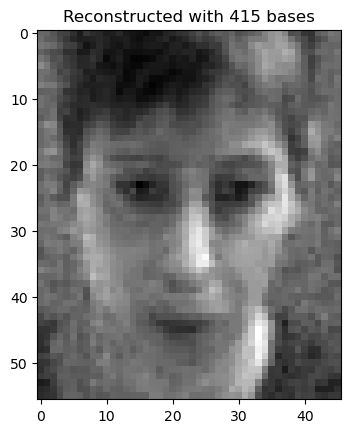
\includegraphics[width=\linewidth]{image/q1_recon_test_415.png}
		\caption{415 bases}
		\label{fig:test_re_415}
	\end{subfigure}
	\caption{Test data reconstruction results}
	\label{fig:recon_test}
\end{figure}

For more detailed analysis, we computed the reconstruction error. The theoretical error is given by $\sum_{i=n+1}^M \lambda_i$ where $n$is the number of bases we used for the reconstruction, $M$is total number of PCA bases, and $\lambda_i$ is eigenvalues of unused eigenvectors. The actual reconstruction error can be calculated using L2-norm of difference between the original and reconstructed data.

\begin{figure}
	\centering
	\begin{subfigure}[t]{0.48\linewidth}
		\centering
		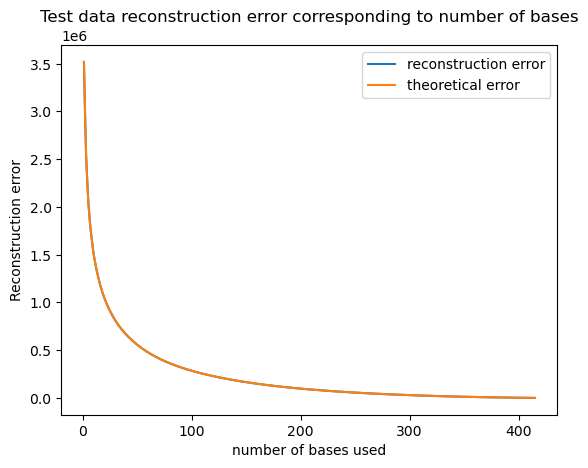
\includegraphics[width=\linewidth]{image/q1_recon_error_train.png}
		\caption{training data}
		\label{fig:recon_error_train}
	\end{subfigure}%
	\hfill
	\begin{subfigure}[t]{0.48\linewidth}
		\centering
		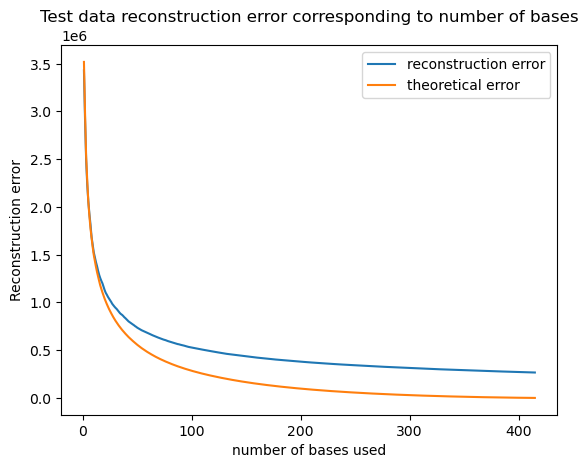
\includegraphics[width=\linewidth]{image/q1_recon_error_test.png}
		\caption{test data}
		\label{fig:recon_error_test}
	\end{subfigure}
	\caption{PCA reconstruction error}
	\label{fig:recon_error}
\end{figure}

As shown in \cref{fig:recon_error}, the reconstruction error from the training data matched the theoretical result. However, for the test data, while the graph’s shape was similar to the theoretical result, the actual values differed slightly. This may be because the PCA bases used for reconstruction were derived from the training data, not the test data.

\subsection{KNN classification using Eigenfaces}

We can also perform classification using PCA with NN classifier. As shown in \cref{fig:q1_knn_accuracy}, accuracy improves with more PCA bases and fewer neighbors($k$). More PCA bases preserve more data information, leading to accurate projections in the PCA subspace. For the number of neighbors, using fewer makes the classifier more sensitive to local information and better at preserving class boundaries, thus increasing classification accuracy.

In terms of time and memory, the number of neighbors made no significant difference. However, as shown in \cref{fig:q1_knn_time} and \cref{fig:q1_knn_memory}, the execution time and memory usage of the k-NN classifier linearly increase  with the number of PCA bases increase. This is because, the execution time and memory usage is $O(N\cdot M)$ where $N$ is the number of total data and $M$ is the number of PCA bases we used. Since $k$ only affects on final selection process, its impact during the computation is very small.

\begin{figure}
	\centering
	
	% 윗줄에 하나의 이미지, 크기는 0.48로 유지
	\begin{subfigure}[t]{0.48\linewidth}
		\centering
		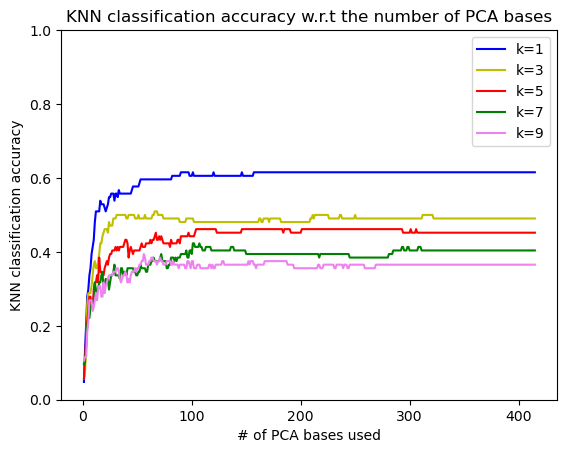
\includegraphics[width=\linewidth]{image/q1_accuracy.png}
		\caption{accuracy}
		\label{fig:q1_knn_accuracy}
	\end{subfigure}
	
    \vspace{0.5cm} % 이미지들 사이에 공간 추가

	% 아랫줄에 두 개의 이미지, 크기 동일하게 0.48
	\begin{subfigure}[t]{0.48\linewidth}
		\centering
		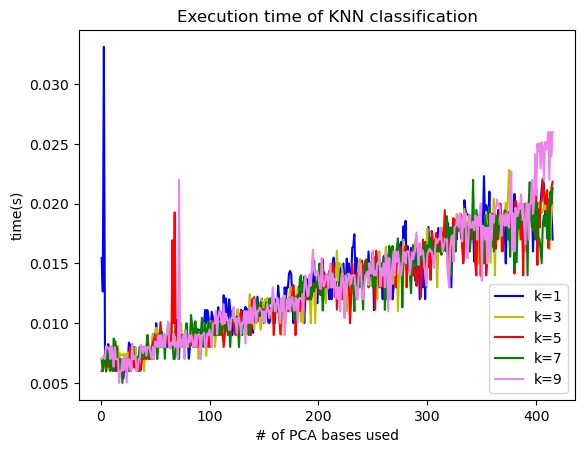
\includegraphics[width=\linewidth]{image/q1_time.png}
		\caption{running time}
		\label{fig:q1_knn_time}
	\end{subfigure}%
	\hfill
	\begin{subfigure}[t]{0.48\linewidth}
		\centering
		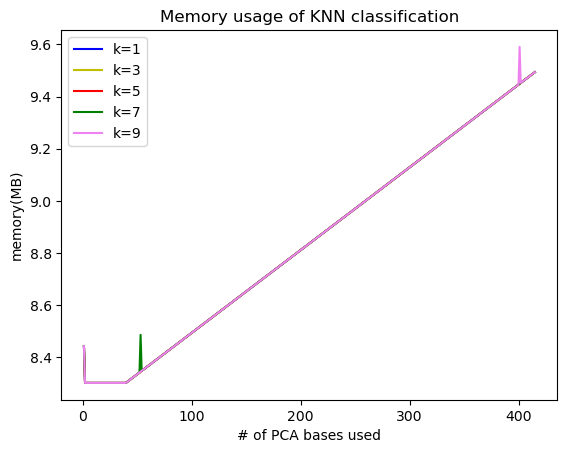
\includegraphics[width=\linewidth]{image/q1_memory.png}
		\caption{memory usage}
		\label{fig:q1_knn_memory}
	\end{subfigure}

	\caption{Analysis on KNN classification using PCA}
	\label{fig:pca_knn}
\end{figure}

However, its overall prediction accyracy is about 0.6, which is not that high. This might because, PCA is not very sophisticated model to capture all the detailed features of data. As we also check from the confusion matrix(\cref{fig:q1_cm}), there are many components outside the diagonal, that failed to be predicted.


Detailed prediction examples can be found in Appendix B, C.